% Opcje klasy 'iithesis' opisane sa w komentarzach w pliku klasy. Za ich pomoca
% ustawia sie przede wszystkim jezyk i rodzaj (lic/inz/mgr) pracy, oraz czy na
% drugiej stronie pracy ma byc skladany wzor oswiadczenia o autorskim wykonaniu.
\documentclass[inz,longabstract]{iithesis}

\usepackage[utf8]{inputenc}

%%%%% DANE DO STRONY TYTUŁOWEJ
% Niezaleznie od jezyka pracy wybranego w opcjach klasy, tytul i streszczenie
% pracy nalezy podac zarowno w jezyku polskim, jak i angielskim.
% Pamietaj o madrym (zgodnym z logicznym rozbiorem zdania oraz estetyka) recznym
% zlamaniu wierszy w temacie pracy, zwlaszcza tego w jezyku pracy. Uzyj do tego
% polecenia \fmlinebreak.
\polishtitle    {Realistyczny rendering krajobrazów leśnych\fmlinebreak generowanych proceduralnie}
\englishtitle   {Realistic rendering of procedural generated forest landscapes}
\polishabstract {Strzeszczenie po polsku\ldots}
\englishabstract{English abstract\ldots}
% w pracach wielu autorow nazwiska mozna oddzielic poleceniem \and
\author         {Bartosz Rudzki}
% w przypadku kilku promotorow, lub koniecznosci podania ich afiliacji, linie
% w ponizszym poleceniu mozna zlamac poleceniem \fmlinebreak
\advisor        {dr Andrzej Łukaszewski}
%\date          {}                     % Data zlozenia pracy
% Dane do oswiadczenia o autorskim wykonaniu
\transcriptnum {291481}                     % Numer indeksu
\advisorgen    {dr Andrzeja Łukaszewskiego} % Nazwisko promotora w dopelniaczu
%%%%%

%%%%% WLASNE DODATKOWE PAKIETY
%
%\usepackage{graphicx,listings,amsmath,amssymb,amsthm,amsfonts,tikz}
\usepackage{graphicx, amsmath, gensymb, float, textcomp}
%
%%%%% WŁASNE DEFINICJE I POLECENIA
\graphicspath{{./pictures/}}
%\theoremstyle{definition} \newtheorem{definition}{Definition}[chapter]
%\theoremstyle{remark} \newtheorem{remark}[definition]{Observation}
%\theoremstyle{plain} \newtheorem{theorem}[definition]{Theorem}
%\theoremstyle{plain} \newtheorem{lemma}[definition]{Lemma}
%\renewcommand \qedsymbol {\ensuremath{\square}}
% ...
%%%%%

\begin{document}

%%%%% POCZĄTEK ZASADNICZEGO TEKSTU PRACY
\chapter{Wprowadzenie}
    Pracy skupia się na zbadaniu i zastosowaniu dwóch pojęć z dziedziny grafiki komputerowej: realistyczny rendering i generowanie proceduralne. 
    
    Pierwsze zagadnienie dotyczy przedstawienia wcześniej przygotowanego modelu w sposób zrozumiały dla człowieka. Modelem może być plik opisujący kształt dzbanka. Przykładowa reprezentacja to zbiór trójkątów rozmieszczonych w przestrzeni z uwzględnieniem dodatkowych informacji takich np. kolor. Rendering takiego modelu polegałby na zamianie wszystkich tych danych na obraz, który mógłby być pokazany człowiekowi. O realistycznym renderingu możemy mówić wtedy, kiedy stworzony przez nas obraz przypomina prawdziwy dzbanek, który chcieliśmy zamodelować. 
    
    Generowanie proceduralne skupia się na tworzeniu modeli przy pomocy algorytmów. Człowiek może wpływać na finalny produkt przy pomocy zmiany parametrów jednak nie uczestniczy w samym procesie tworzenia. Jest to bardzo wydajna metoda pozwalająca na tworzenie nieskończenie wielu różnych modeli o zadanych właściwościach jak np. rośliny.
    
    Celem programu napisanego w ramach tej pracy jest generowanie prostego krajobrazu leśnego, a następnie względnie realistyczny rendering stworzonego środowiska. Sam program jest wysoce sparametryzowany, dzięki czemu użytkownik może realnie wpływać na finalny rezultat.
    
\chapter{Zastosowane rozwiązania}
    \section{Generowanie proceduralne}
        \subsection{Rośliny}
            Kształt roślin posiada wiele regularności. Dzięki temu można opisać je przy pomocy tak zwanych L-systemów. Jest to sposób reprezentacji modelu pod postacią zestawu reguł tworzących gramatykę. Zaczynając od jednego symbolu jesteśmy wstanie wygenerować zbiór symboli - słowo. Osiągamy to poprzez zdefiniowanie dodatniej liczby różnych produkcji. Są to reguły zamieniania wybranego symbolu na słowo. Przykładowy L-System może wyglądać następująco:
            \begin{align*}
                axiom &: \alpha \\
                prod1 &: \alpha \rightarrow \alpha\beta\alpha \\
                prod2 &: \beta \rightarrow \beta\beta
            \end{align*}
            Produkcje aplikowane są jednocześnie w obrębie jednej iteracji. Podając liczbę iteracji możemy generować coraz dłuższe ciągi. Dla N = 1 otrzymujemy $\alpha\beta\alpha$, a dla N = 2 mamy $\alpha\beta\alpha\beta\beta\alpha\beta\alpha$.
            
            Finalnym produktem L-systemu jest słowo, które możemy potraktować jako polecenia dla rysującego żółwia. Żółw czytając słowo od lewej do prawej będzie interpretować każdy symbol jako komendę. Przykłady poleceń to: idź prosto rysując linię albo skręć w lewo o wcześniej ustalony kąt. W przypadku gdy żółw nie zna symbolu nie robi nic i czyta dalej. Rysunek \ref{fig:turtleExample} przedstawia przykładową interpretację słowa $\alpha\beta\alpha\beta\beta\alpha\beta\alpha$ gdzie $\alpha$ to idź naprzód, a $\beta$ skręć w lewo o 30\degree.
            \begin{figure}[H]
                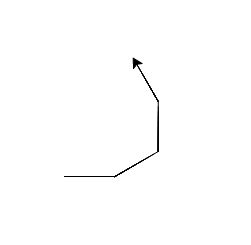
\includegraphics[width=\linewidth]{turtleExample.png}
                \caption{Interpretacja dla słowa $\alpha\beta\alpha\beta\beta\alpha\beta\alpha$, gdzie $\alpha$ to idź naprzód, a $\beta$ skręć w lewo o 30\degree.}
                \label{fig:turtleExample}
            \end{figure}
            
            Aby żółw był wstanie rysować rośliny potrzebujemy symbol pozwalający się rozgałęziać. Można osiągnąć to poprzez dodanie stosu pamiętającego aktualny stan żółwia oraz symbole na nim operujące:
            \begin{description}
                \item[{[}] - odłóż aktualny stan na stos
                \item[{]}] - ściągnij i zaaplikuj stan z góry stosu 
            \end{description}
            Stanem żółwia jest wszystko co zmienia się przy pomocy symboli np. pozycja, orientacja lub długość rysowanej linii. Rysunek \ref{fig:lsystemPlants} pokazuje przykładowe L-systemy z książki \textit{The Algorithmic Beauty of Plants}\cite{plants}, które używają symboli tworzących rozgałęzienia. 
            \begin{figure}[H]
                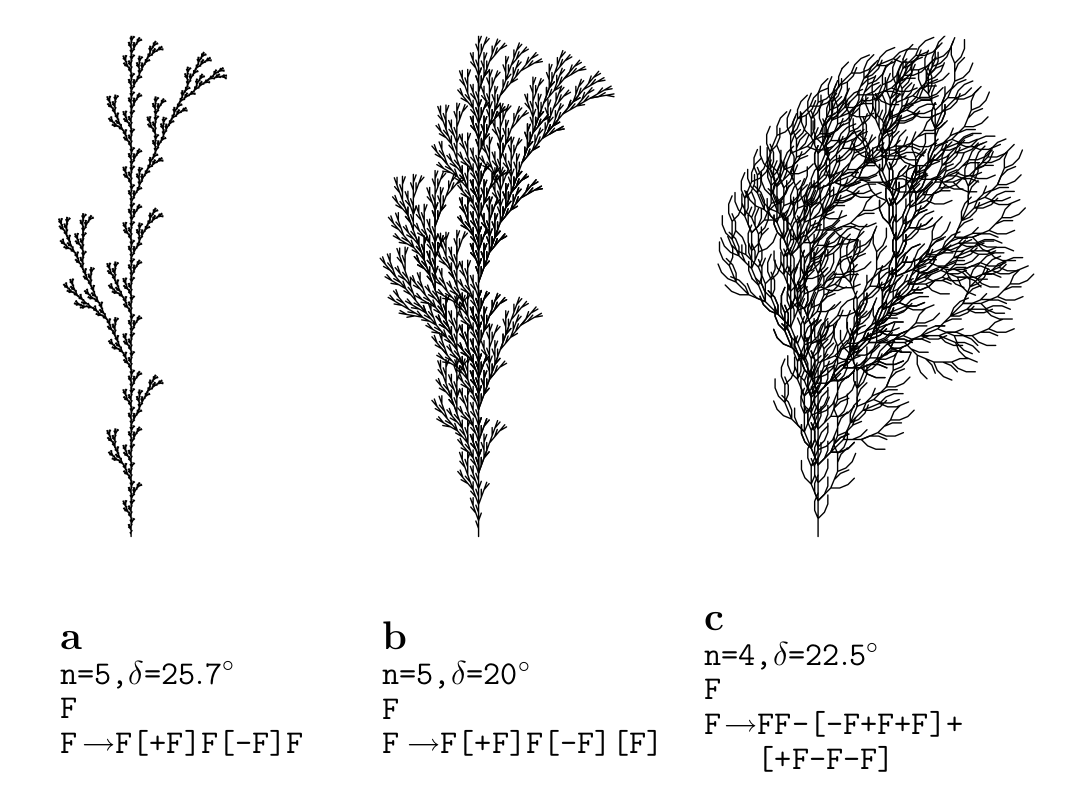
\includegraphics[width=\linewidth]{lsystemPlants.png}
                \caption{Przykład użycia symboli operujących na stosie\cite{plants}} 
                \label{fig:lsystemPlants}
            \end{figure}
            
            Wspomniana wcześniej książka Prusinkiewicza i Lindenmayer'a\cite{plants} dokładnie opisuje L-systemy jako zagadnienie naukowe oraz podaje wiele przykładów produkcji tworzących realistycznie wyglądające rośliny. Część z nich wymaga bardziej zaawansowanych technik produkcji symbolów np. L-systemy parametryczne. Do tej pory zakładaliśmy, że wszystkie parametry (np. kąt skrętu, długość kroku) były ustalone na początku i nie zmieniały się. Parametryzując symbole i produkcje możemy wpływać lepiej na finalny kształt. Ma to zastosowanie między innymi w generowaniu drzew. Rysunek \ref{fig:hondaTrees} przedstawia produkcje drzew wymyślonych przez Hondę\cite{honda}, a pokazanych u Prusinkiewicza\cite{plants}.
            \begin{figure}[H]
                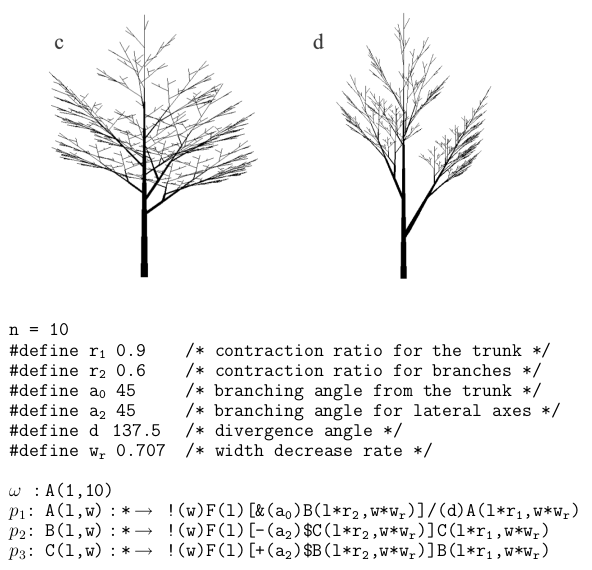
\includegraphics[width=\linewidth]{hondaTrees.png}
                \caption{L-system parametryczny generujący drzewa \cite{plants}\cite{honda}} 
                \label{fig:hondaTrees}
            \end{figure}
            
            L-systemy mogę również generować wielokąty. Jest to szczególnie przydatne w tworzeniu liści. Rysunek \ref{fig:lsystemLeafs} prezentuje kilka rodzajów liści wygenerowanych z jednego L-systemu. Możliwe jest to dzięki wprowadzeniu nowych symboli:
            \begin{description}
                \item[\texttt{\{}] - zacznij tworzyć nowy wielokąt 
                \item[.] - zapisz aktualną pozycję jako wierzchołek
                \item[\texttt{\}}] - zakończ aktualny wielokąt
            \end{description}
            \begin{figure}[H]
                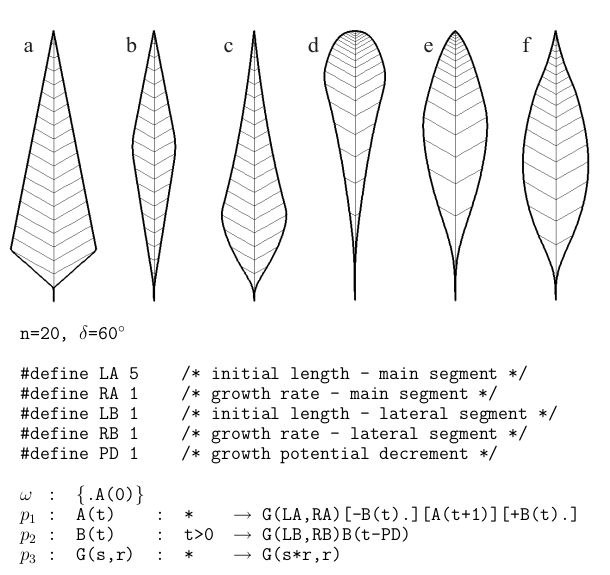
\includegraphics[width=\linewidth]{lsystemLeafs.png}
                \caption{L-system parametryczny generujący liście \cite{plants}} 
                \label{fig:lsystemLeafs}
            \end{figure}
            
            Wcześniej opisane zastosowania L-systemów pokazują dlaczego jest to idealny kandydat do tworzenia realistycznych modeli roślin. Różnorodność definiowanych kształtów, rozbudowywanie funkcjonalności poprzez dodawanie nowych symboli oraz łatwe parametryzowanie to jedne z wielu zalet tej techniki. Wszystko to sprawia, że L-systemy są często wykorzystywane w wielu różnych projektach - również w tym. 
            
        \subsection{Teren}
            Problem generowania terenu można sprowadzić do problemu generowania mapy wysokości. Jest to macierz wypełniona liczbami reprezentującymi wysokość wybranych punktów. Owe punkty pomiaru rozłożone są równomiernie na osi X i Z. Mając taką macierz w łatwy sposób jesteśmy wstanie wygenerować teren - tworzymy kwadraty dla każdej czwórki sąsiadujących punktów - patrz rysunek \ref{fig:heightmap}. 
            \begin{figure}[H]
                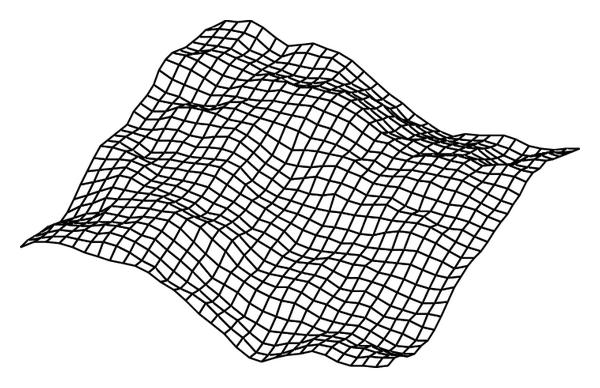
\includegraphics[width=\linewidth]{heightmap.png}
                \caption{Przykładowy teren wygenerowany przy użyciu mapy wysokości\cite{heightmap}} 
                \label{fig:heightmap}
            \end{figure}
            
            Istnieje wiele algorytmów generujących mapy wysokości. Mój wybór padł na tak zwany \textit{Diamond-square algorithm}. Dla ustalonego N generuje on mapę wysokości o rozmiarze $2^N$+1 x $2^N$+1. Na początku ustala się wartości w rogach macierzy. Następnie wykonuje się na przemiennie fazę diamond i square, aż do ustalenia wszystkich wysokości. 
            
            Faza diamond polega na wygenerowaniu wysokości w środku każdego kwadratu, który nie ma ustalonej tej wartości. Faza square robi to samo tylko, ze dla punktów tworzących kształt rombu. Rysunek \ref{fig:diamondSquare} obrazuje przebieg algorytmu. 
            \begin{figure}[H]
                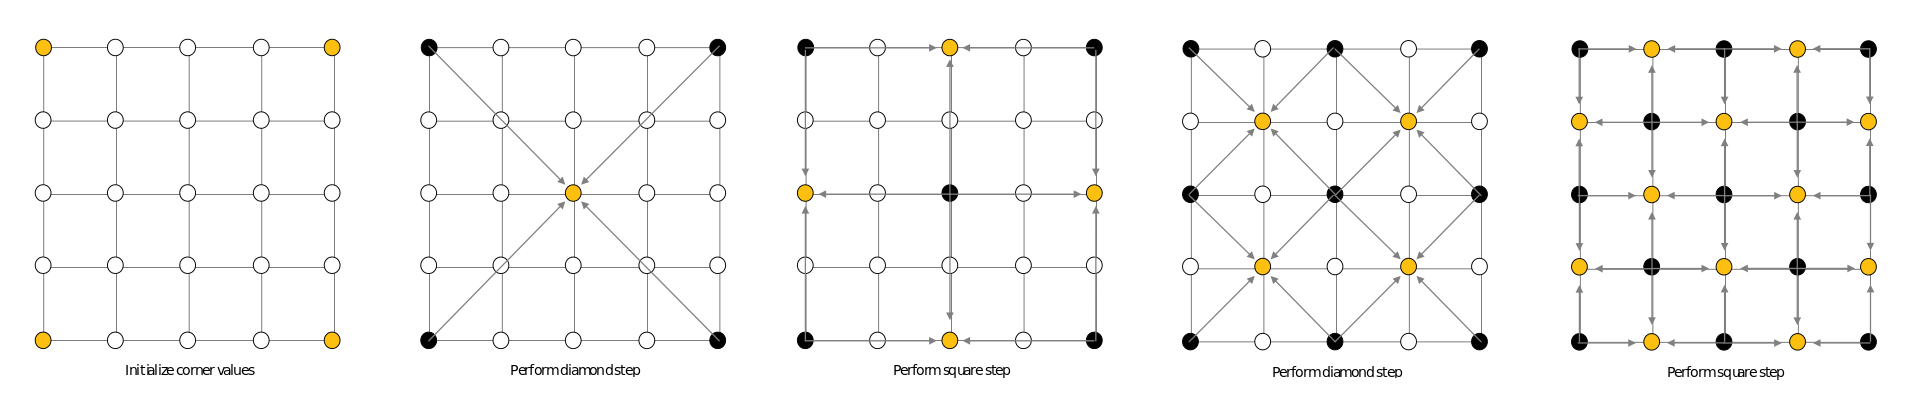
\includegraphics[width=\linewidth]{diamondSquare.png}
                \caption{Przebieg algorytmu diamond-square dla N = 2.} 
                \label{fig:diamondSquare}
            \end{figure}
            
            Obliczanie nowej wartości w środku polega na wzięciu średniej z wysokości wierzchołków tworzących kształt (kwadrat, romb). Dodatkowo dodajemy do obliczanej wartości pewien czynnik losowy, z przedziału (-X, X) dla ustalonego X. Dla każdej kolejnej pary faz ów czynnik jest zmniejszany poprzez przemnożenie go przez pewne $R < 1$.
            
            \textit{Diamond-square algorithm} jest zarówno prosty jak i efektywny. Ustalając kilka parametrów jesteśmy wstanie tworzyć bardzo różnorodny teren. 
            
        \subsection{Tekstury}
            Mając wygenerowany model - kształt,  musimy nadać mu również kolor. Jednym z założeniem programu było w pełni proceduralne podejście. Dotyczy to również tekstur. Każda tekstura w programie opisywana jest przez materiał. Materiał oblicza kolor na podstawie funkcji \textit{calcDiffuse(pos3D) \textrightarrow color}, gdzie $pos3D$ to pozycja w świecie. W celu uproszczenia i ujednolicenia systemu zdecydowałem się zaimplementować jeden wzór, który został zastosowany do każdego materiału. Wygląda on następująco:
            \begin{gather*}
                calcDiffuse(pos3D) = mix(color1, color2, factor) \\
                gdzie \\
                factor = clamp(noise(pos3D * posF) * valF, 0, 1)
            \end{gather*}
            

            Finalny kolor to mieszanka $color1$ i $color2$ w stosunku $1 - factor$ i $factor$. Sam $factor$ to odpowiednio obliczona wartość szumu Perlina. Dzięki $posF$ możemy skalować szum, a dzięki $valF$ możemy wymuszać faworyzowanie wartości bliższych 0 albo 1.
            
            Jedynym materiałem w programie odbiegającym od tej metody jest materiał terenu. Łączy on ze sobą dwa inne materiały - grunt i skały. Do pewnej ustalonej wysokości kolor obliczany jest tylko dla gruntu. Analogicznie powyżej pewnego poziomu stosuję tylko kolor skał. Po środku dochodzi do mieszania kolorów w stosunku zależnym od odległości do ustalonych granic:
            \begin{gather*}
            mix(calcRockColor(pos), calcGroundColor(pos), groundFactor) \\
            gdzie \\
            groundFactor = (groundEndY - posY) / (groundEndY - rockStartY) \\
            \end{gather*}
            
            Zaprezentowane rozwiązanie okazało się wystarczające, aby osiągnąć zadowalające rezultaty. Jest łatwe do implementacji, ujednolicone dla użytkownika oraz na tyle rozbudowane aby wyrażać niebanalną kolorystkę.
            
        \subsection{Rozmieszczanie roślin}
        \subsection{Umiejscawianie kamery}
    \section{Realistyczny rendering}
        \subsection{Pathtracer}
        \subsection{Niebo}
        \subsection{Słońce}
        
\chapter{Poradnik użytkowania}

\chapter{Szczegóły programistyczne}

\chapter{Przykłady użycia}

%%%%% BIBLIOGRAFIA

\bibliographystyle{unsrt}
\bibliography{bibliography}

%\begin{thebibliography}{1}
%\bibitem{example} \ldots
%\end{thebibliography}

\end{document}
